\chapter{Processes, the Kernel, and System Calls}

\section{The process abstraction}

\begin{definition}[Process]
A \textbf{process} is an environment in which an application program runs. It consists of
\begin{itemize}
  \item one or more \textbf{threads};
  \item a virtual memory \textbf{address space} (code, data, heap, stacks);
  \item other resources: open file descriptors, current working directory, process ID,
    parent/child relationships, credentials.
\end{itemize}
\end{definition}

Processes are \textbf{isolated} from each other: one process cannot read another's memory or
files descriptors unless the kernel explicitly allows sharing. The kernel keeps per-process state
in a process control block (\code{struct proc} in OS/161).

\begin{lstlisting}[style=c]
struct proc {                       /* kern/include/proc.h (with A2 additions) */
    char *p_name;
    struct spinlock p_lock;
    struct threadarray p_threads;   /* threads in this process */
    struct addrspace *p_addrspace;  /* virtual address space */
    struct vnode *p_cwd;            /* current directory */
    /* added for assignment 2: */
    pid_t p_pid;
    struct proc *p_parent;
    int p_exitcode; bool p_exited;
    struct cv *p_waitcv;
};
\end{lstlisting}

\section{Process management system calls}

\begin{center}
\begin{tabular}{@{}lll@{}}
\toprule
Operation & Linux / POSIX & OS/161 \\
\midrule
Create & \code{fork}, \code{clone} & \code{fork} \\
Replace program & \code{execve} & \code{execv} \\
Terminate & \code{\_exit}, \code{exit} & \code{\_exit} \\
Wait for child & \code{waitpid}, \code{wait} & \code{waitpid} \\
Identity & \code{getpid}, \code{getppid} & \code{getpid} \\
\bottomrule
\end{tabular}
\end{center}

\begin{description}
  \item[\code{fork()}] creates a new process (the \emph{child}) that is a \emph{clone} of the
    caller (the \emph{parent}): a copy of the address space, same open files, one thread that
    starts executing by returning from \code{fork}. Returns the child's PID in the parent and
    0 in the child.
  \item[\code{\_exit(code)}] terminates the calling process. Its exit status is kept until the
    parent collects it; a terminated-but-uncollected process is a \textbf{zombie}.
  \item[\code{waitpid(pid, \&status, options)}] blocks until child \code{pid} has exited and
    returns its exit status. A process may only wait for its own children.
  \item[\code{execv(path, argv)}] replaces the calling process's address space with a new
    program loaded from \code{path}, passing arguments \code{argv}. The PID, open files, and
    parent/child relationships stay the same. On success it does not return.
\end{description}

\begin{example}[The classic fork/exec/wait pattern]
\begin{lstlisting}[style=c]
int main(void) {
    pid_t pid = fork();
    if (pid < 0) { perror("fork"); _exit(1); }
    if (pid == 0) {                       /* child */
        char *args[] = { "/bin/ls", "-l", NULL };
        execv(args[0], args);
        _exit(127);                       /* only reached if execv failed */
    }
    int status;                           /* parent */
    waitpid(pid, &status, 0);
    printf("child exited with %d\n", WEXITSTATUS(status));
    return 0;
}
\end{lstlisting}
\end{example}

\begin{figure}[H]
\centering
\begin{tikzpicture}[x=1cm, y=1cm, font=\small, >=Stealth]
  \node[anchor=east] at (-0.1,1.5) {parent};
  \node[anchor=east] at (-0.1,0) {child};
  \draw[line width=4pt, blue!50] (0,1.5) -- (2,1.5);
  \draw[line width=4pt, blue!50, dash pattern=on 3pt off 2pt] (3,1.5) -- (8.6,1.5);
  \draw[line width=4pt, blue!50] (2,1.5) -- (3,1.5);
  \draw[line width=4pt, blue!50] (8.6,1.5) -- (10.4,1.5);
  \draw[->, thick] (2,1.4) -- (2,0.15);
  \node[font=\scriptsize, anchor=south] at (2,1.7) {\code{fork()}};
  \node[font=\scriptsize, anchor=south] at (3,1.7) {\code{waitpid}};
  \node[font=\scriptsize, anchor=south] at (5.8,1.7) {blocked};
  \draw[line width=4pt, green!50!black!50] (2,0) -- (3.4,0);
  \draw[line width=4pt, orange!60] (3.4,0) -- (8.5,0);
  \node[font=\scriptsize, anchor=north] at (3.4,-0.2) {\code{execv("/bin/ls")}};
  \node[font=\scriptsize] at (6,0.3) {running \code{ls}};
  \node[font=\scriptsize, anchor=north] at (8.5,-0.2) {\code{\_exit}};
  \draw[->, thick, red!70!black] (8.5,0.15) -- node[right, font=\scriptsize]{exit status} (8.6,1.35);
  \draw[->] (0,-0.9) -- (10.6,-0.9) node[right, font=\scriptsize]{time};
\end{tikzpicture}
\caption{The fork/exec/wait pattern over time: the child replaces its
program with \code{ls}; the parent sleeps in \code{waitpid} until the
child's \code{\_exit} hands back the status.}
\end{figure}

\begin{example}[Counting forks]
\code{for (i = 0; i < 3; i++) fork();} creates $2^3 = 8$ processes in total (7 new), since
every existing process doubles at each iteration.
\end{example}

\begin{figure}[H]
\centering
\begin{tikzpicture}[font=\scriptsize, >=Stealth,
  pr/.style={circle, draw, thick, minimum size=6mm, inner sep=0pt},
  level distance=1.1cm,
  level 1/.style={sibling distance=4.2cm},
  level 2/.style={sibling distance=2.1cm},
  level 3/.style={sibling distance=1.05cm},
  edge from parent/.style={draw, thick, ->}]
  \node[pr, fill=gray!20] {P}
    child {node[pr] {P}
      child {node[pr] {P} child {node[pr] {P}} child {node[pr, fill=blue!15] {}}}
      child {node[pr, fill=blue!15] {} child {node[pr, fill=blue!15] {}} child {node[pr, fill=blue!15] {}}}}
    child {node[pr, fill=blue!15] {}
      child {node[pr, fill=blue!15] {} child {node[pr, fill=blue!15] {}} child {node[pr, fill=blue!15] {}}}
      child {node[pr, fill=blue!15] {} child {node[pr, fill=blue!15] {}} child {node[pr, fill=blue!15] {}}}};
  \node[anchor=west] at (4.6,-1.1) {after $i=0$: 2 processes};
  \node[anchor=west] at (4.6,-2.2) {after $i=1$: 4};
  \node[anchor=west] at (4.6,-3.3) {after $i=2$: 8};
\end{tikzpicture}
\caption{Each \code{fork} splits one process into two (left branch: the
caller continuing, right branch: its new child, shaded). The leaves are the
8 processes alive at the end; the original process P follows the leftmost
path.}
\end{figure}

\section{System calls}

A system call is the interface between user programs and the kernel. User code cannot call
kernel functions directly (different privilege level, kernel memory is protected), so it executes
a special trap instruction.

\subsection{How a system call works on MIPS / OS/161}
\begin{enumerate}
  \item The application calls a library wrapper, e.g.\ \code{fork()} in \code{libc}.
  \item The wrapper puts the \textbf{system call code} in register \code{v0} (e.g.\
    \code{SYS\_fork}), arguments in \code{a0}--\code{a3} (more on the user stack), and executes
    \code{syscall}.
  \item \code{syscall} raises an exception: the CPU switches to kernel mode, records the cause
    (\code{EX\_SYS}) and the faulting PC in coprocessor 0 registers, and jumps to the fixed
    exception handler address.
  \item The kernel saves the user's registers in a \textbf{trapframe} on the thread's kernel
    stack and calls \code{mips\_trap} $\to$ \code{syscall(tf)}, which dispatches on
    \code{tf->tf\_v0}.
  \item The result is placed in the trapframe: \code{v0} = return value (or error code),
    \code{a3} = 0 for success / 1 for failure. The PC in the trapframe is advanced by 4 so the
    \code{syscall} instruction is not re-executed.
  \item The kernel restores registers from the trapframe and executes \code{rfe}/\code{jr}
    to return to user mode. The libc wrapper checks \code{a3}; on failure it stores \code{v0}
    into \code{errno} and returns $-1$.
\end{enumerate}

\begin{figure}[H]
\centering
\begin{tikzpicture}[font=\scriptsize, >=Stealth, node distance=0.35cm,
  st/.style={draw, rounded corners, align=center, minimum height=0.9cm, text width=2.4cm}]
  \fill[blue!6] (-1.4,-0.95) rectangle (11.4,-3.25);
  \node[font=\scriptsize, anchor=west] at (-1.25,-3.05) {kernel mode};
  \node[font=\scriptsize, anchor=west] at (-1.25,0.6) {user mode};
  \node[st] (app) at (0,0) {application\\calls \code{fork()}};
  \node[st] (lib) at (3.3,0) {libc stub: \code{v0}${}\gets{}$\code{SYS\_fork}; \code{syscall}};
  \node[st] (exc) at (3.3,-2) {\code{common\_exception}: save trapframe};
  \node[st] (trap) at (6.6,-2) {\code{mips\_trap}\\$\to$ \code{syscall(tf)}};
  \node[st] (sys) at (9.9,-2) {\code{sys\_fork};\\set \code{v0}, \code{a3}, \code{epc+=4}};
  \node[st] (ret) at (9.9,0) {back in libc: check \code{a3}, return};
  \draw[->, thick] (app) -- (lib);
  \draw[->, thick, red!70!black] (lib) -- node[right]{trap} (exc);
  \draw[->, thick] (exc) -- (trap);
  \draw[->, thick] (trap) -- (sys);
  \draw[->, thick, red!70!black] (sys) -- node[left]{restore trapframe, \code{rfe}} (ret);
\end{tikzpicture}
\caption{The path of a system call on OS/161: the trap switches to kernel
mode and the kernel stack, and the return restores the saved user state.}
\end{figure}

\begin{lstlisting}[style=mips]
# user-level stub generated for each system call (userland/lib/libc/syscalls.S)
reboot:
    j    __syscall
    addiu v0, $0, SYS_reboot     # delay slot: syscall number in v0
__syscall:
    syscall                      # trap into the kernel
    beq  a3, $0, 1f              # a3 == 0 -> success
    nop
    sw   v0, errno               # failure: set errno
    li   v1, -1
    li   v0, -1                  # return -1
1:  j    ra
    nop
\end{lstlisting}

\begin{lstlisting}[style=c]
/* kern/arch/mips/syscall/syscall.c (abbreviated) */
void syscall(struct trapframe *tf) {
    int callno = tf->tf_v0, err;
    int32_t retval = 0;
    switch (callno) {
    case SYS_getpid:  err = sys_getpid((pid_t *)&retval); break;
    case SYS_fork:    err = sys_fork(tf, (pid_t *)&retval); break;
    case SYS__exit:   sys__exit((int)tf->tf_a0); panic("unreachable");
    case SYS_waitpid: err = sys_waitpid((pid_t)tf->tf_a0, (userptr_t)tf->tf_a1,
                                        (int)tf->tf_a2, (pid_t *)&retval); break;
    default:          err = ENOSYS; break;
    }
    if (err) { tf->tf_v0 = err;    tf->tf_a3 = 1; }
    else     { tf->tf_v0 = retval; tf->tf_a3 = 0; }
    tf->tf_epc += 4;              /* skip over the syscall instruction */
}
\end{lstlisting}

\begin{important}[Never trust user pointers]
A pointer passed as a system call argument (e.g.\ \code{status} in \code{waitpid}) is a
\emph{user} virtual address. It might be NULL, point into the kernel, or be unmapped. The kernel
must use \code{copyin}/\code{copyout} (and \code{copyinstr}), which validate the address and
handle faults gracefully, returning \code{EFAULT} instead of crashing the kernel.
\end{important}

\section{Exceptions and interrupts}

\begin{definition}
An \textbf{exception} is a synchronous event caused by the current instruction (system call,
arithmetic overflow, illegal instruction, address error, TLB miss/fault). An \textbf{interrupt}
is an asynchronous event raised by a device (timer, disk, network, serial console).
\end{definition}

On MIPS R3000 both are handled the same way: the processor switches to kernel mode, disables
interrupts, saves the PC in \code{EPC}, records the reason in the \code{Cause} register, and
jumps to a fixed address: \code{0x80000000} for user-mode TLB misses (UTLB), \code{0x80000080}
for everything else. OS/161 exception codes include:

\begin{center}
\begin{tabular}{@{}cll@{}}
\toprule
Code & Name & Meaning \\
\midrule
0 & \code{EX\_IRQ} & interrupt \\
1 & \code{EX\_MOD} & write to a read-only TLB page \\
2, 3 & \code{EX\_TLBL}, \code{EX\_TLBS} & TLB miss on load / store \\
4, 5 & \code{EX\_ADEL}, \code{EX\_ADES} & address error on load / store \\
8 & \code{EX\_SYS} & system call \\
10 & \code{EX\_RI} & reserved (illegal) instruction \\
12 & \code{EX\_OVF} & arithmetic overflow \\
\bottomrule
\end{tabular}
\end{center}

\subsection{Trapframes vs switchframes}
\begin{itemize}
  \item The \textbf{trapframe} is built by the exception handler (\code{common\_exception}) and
    saves \emph{all} general registers plus \code{EPC}, \code{Cause}, \code{Status},
    \code{hi}/\code{lo}, because the interrupted code had no warning.
  \item The \textbf{switchframe} is built by \code{switchframe\_switch} during a context switch
    and holds only callee-saved registers (Ch.~2).
\end{itemize}

\subsection{Kernel stacks}
Each thread has \emph{two} stacks: a user stack (in the process's address space, used while
running user code) and a \textbf{kernel stack} (in kernel memory, used while running in the
kernel on that thread's behalf). On an exception the handler switches \code{sp} to the thread's
kernel stack before saving anything. Reasons: the user stack pointer might be invalid or
malicious, and kernel data must not be visible to user code.

\begin{center}
\begin{tikzpicture}[f/.style={draw,text width=4.8cm,align=center,minimum height=0.6cm,font=\small}]
  \node[f,fill=gray!10] (a) {trapframe (all user registers)};
  \node[f,above=0pt of a] (b) {\code{mips\_trap} frame};
  \node[f,above=0pt of b] (c) {\code{syscall} frame};
  \node[f,above=0pt of c] (d) {\code{sys\_waitpid} \ldots};
  \node[f,above=0pt of d] (e) {\code{cv\_wait}, \code{thread\_switch}};
  \node[f,above=0pt of e,fill=blue!8] (g) {switchframe};
  \node[left=0.3cm of a,font=\small,align=right] {bottom of\\kernel stack};
  \node[left=0.3cm of g,font=\small,align=right] {top (sp)};
\end{tikzpicture}
\end{center}
Kernel stack of a thread that made a \code{waitpid} system call and blocked.

\section{Implementing fork, waitpid, \_exit in OS/161}

\subsection*{\code{sys\_fork}}
\begin{enumerate}
  \item Create a new \code{struct proc} (\code{proc\_create\_runprogram}), assign a PID.
  \item Copy the parent's address space with \code{as\_copy}.
  \item Record parent/child relationship.
  \item Copy the parent's trapframe to the heap (the parent's kernel stack may change before
    the child runs).
  \item \code{thread\_fork} a child thread whose entry function (\code{enter\_forked\_process})
    copies the trapframe onto its own kernel stack, sets \code{v0 = 0}, \code{a3 = 0},
    \code{epc += 4}, activates the address space, and calls \code{mips\_usermode} to return to
    user mode.
  \item Parent returns the child's PID.
\end{enumerate}

\subsection*{\code{sys\_waitpid} and \code{sys\_\_exit}}
\begin{lstlisting}[style=c]
void sys__exit(int exitcode) {
    struct proc *p = curproc;
    lock_acquire(proc_table_lock);
    p->p_exitcode = _MKWAIT_EXIT(exitcode);
    p->p_exited = true;
    cv_broadcast(p->p_waitcv, proc_table_lock);   /* wake a waiting parent */
    /* children of p become orphans; destroy those already exited */
    lock_release(proc_table_lock);
    as_deactivate();
    as_destroy(proc_getas(p));                    /* free memory now */
    proc_remthread(curthread);
    /* if parent already exited, nobody can wait: destroy p entirely */
    thread_exit();
}

int sys_waitpid(pid_t pid, userptr_t status, int options, pid_t *retval) {
    struct proc *child = proc_lookup(pid);
    if (options != 0) return EINVAL;
    if (child == NULL) return ESRCH;
    if (child->p_parent != curproc) return ECHILD;
    lock_acquire(proc_table_lock);
    while (!child->p_exited)
        cv_wait(child->p_waitcv, proc_table_lock);
    int code = child->p_exitcode;
    lock_release(proc_table_lock);
    int err = copyout(&code, status, sizeof(int));
    if (err) return err;
    *retval = pid;
    return 0;
}
\end{lstlisting}

\subsection*{\code{sys\_execv}}
\begin{enumerate}
  \item Copy the program path and the argument strings from the \emph{old} address space into
    kernel memory (\code{copyinstr}) --- the old address space is about to vanish.
  \item Open the executable (\code{vfs\_open}), create a new address space, activate it, and
    load the ELF file (\code{load\_elf}).
  \item Define the user stack (\code{as\_define\_stack}); copy the argument strings and then the
    \code{argv} pointer array onto the new stack, keeping pointers 4-byte aligned (8-byte aligned
    stack top), with \code{argv[argc] = NULL}.
  \item Destroy the old address space; call \code{enter\_new\_process(argc, argv\_uaddr, sp,
    entrypoint)}, which never returns.
\end{enumerate}

\section{MIPS R3000 essentials for OS/161}
\begin{itemize}
  \item 32 general registers: \code{zero}, \code{at}, \code{v0--v1} (return values / syscall
    number), \code{a0--a3} (arguments), \code{t0--t9} (caller-saved), \code{s0--s8}
    (callee-saved), \code{k0--k1} (reserved for the kernel's exception handler), \code{gp},
    \code{sp}, \code{ra}.
  \item Coprocessor 0 holds system registers: \code{Status} (interrupt enable, user/kernel mode
    bits in a small stack), \code{Cause}, \code{EPC}, \code{BadVAddr}, TLB registers
    (\code{EntryHi}, \code{EntryLo}, \code{Index}).
  \item Branch and jump delay slots, and a load delay slot: the instruction after a branch
    always executes.
  \item 32-bit virtual addresses split into segments: \code{kuseg} (0x00000000--0x7fffffff,
    user, TLB-mapped), \code{kseg0} (0x80000000--0x9fffffff, kernel, cached, direct-mapped to
    physical by subtracting 0x80000000), \code{kseg1} (0xa0000000--0xbfffffff, kernel,
    uncached, direct-mapped; used for devices), \code{kseg2} (kernel, TLB-mapped, unused in
    OS/161).
\end{itemize}

\begin{figure}[H]
\centering
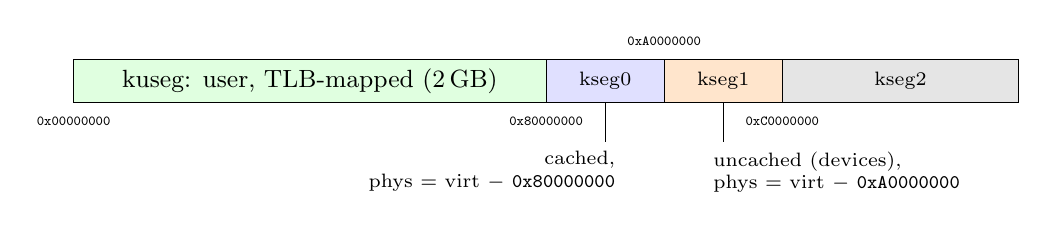
\begin{tikzpicture}[x=1cm, y=0.55cm, font=\small]
  \draw[fill=green!12] (0,0) rectangle (6,1); \node at (3,0.5) {\code{kuseg}: user, TLB-mapped (2\,GB)};
  \draw[fill=blue!12] (6,0) rectangle (7.5,1); \node[font=\scriptsize] at (6.75,0.5) {\code{kseg0}};
  \draw[fill=orange!20] (7.5,0) rectangle (9,1); \node[font=\scriptsize] at (8.25,0.5) {\code{kseg1}};
  \draw[fill=gray!20] (9,0) rectangle (12,1); \node[font=\scriptsize] at (10.5,0.5) {\code{kseg2}};
  \foreach \x/\a in {0/0x00000000, 6/0x80000000, 9/0xC0000000}
    \node[font=\ttfamily\tiny, anchor=north] at (\x,-0.1) {\a};
  \node[font=\ttfamily\tiny, anchor=south] at (7.5,1.1) {0xA0000000};
  \node[font=\scriptsize, align=right, anchor=north east] at (7.0,-0.9) {cached,\\phys $=$ virt $-$ \texttt{0x80000000}};
  \node[font=\scriptsize, align=left, anchor=north west] at (8.0,-0.9) {uncached (devices),\\phys $=$ virt $-$ \texttt{0xA0000000}};
  \draw (6.75,-0.9) -- (6.75,0); \draw (8.25,-0.9) -- (8.25,0);
\end{tikzpicture}
\caption{The MIPS R3000 virtual address space (not to scale). Only
\code{kuseg} and \code{kseg2} go through the TLB; \code{kseg0} and
\code{kseg1} both map onto the first 512\,MB of physical memory.}
\end{figure}

\section{Inter-process communication (brief)}
Processes are isolated, so cooperation needs kernel-provided mechanisms: pipes, files, signals,
shared memory regions, message queues, and sockets (which also work across machines). In W18 this
material was listed as not covered; it appears here only for context.

\section*{Summary}
\begin{itemize}
  \item A process = threads + address space + resources, isolated by the kernel.
  \item \code{fork} clones, \code{execv} replaces the program, \code{\_exit} terminates (zombie
    until collected), \code{waitpid} collects a child's status.
  \item System calls enter the kernel via a trap; the kernel saves a trapframe on the thread's
    kernel stack, dispatches on \code{v0}, returns results in \code{v0}/\code{a3}, and advances
    \code{EPC}.
  \item Exceptions are synchronous, interrupts asynchronous; both use the same entry path on
    MIPS.
  \item Always validate user pointers with \code{copyin}/\code{copyout}.
\end{itemize}
